%%This is a very basic article template.
%%There is just one section and two subsections.
\documentclass[a4paper]{article}
\usepackage{a4wide}
\usepackage{amsmath}
\usepackage{float}
\usepackage{graphicx}
\usepackage{listings}
\usepackage{tikz}

\begin{document}

\title{Exercises on Sequence Labeling}
\author{Charalampos Kaidos}

\maketitle

\section*{Exercise 3}

On figure (figure~\ref{fig:latice},p.~\pageref{fig:latice}) we have designed the
latice of the Viterbi decoder. 

On the horizontal axis we see the k different words of the sentence under check
($t_1 - t_k$). That is the length of the Hidden Markov Model.

On the vertical axis we see the different tokens that are possible at each level
of the HMM ($t^1 - t^{|V|}$). These tokens are words from the vocabulary and are
the states of the HMM.

Finally on top we see the actual words that were observed ($w_1 - w_k$).

On the edges we see the probabilities of transitioning from one node of the
latice to another one (e.g. $P(t_2^1|t_1^3)$). Finally we see the probabilities
of each word observed on the text given that the real word is $t^i$ (e.g.
$P(w_2|t_2^6)$). Note that not all edges and probabilities are drawn to preserve
space and readability of the graph.

\begin{figure}[H]
\centering
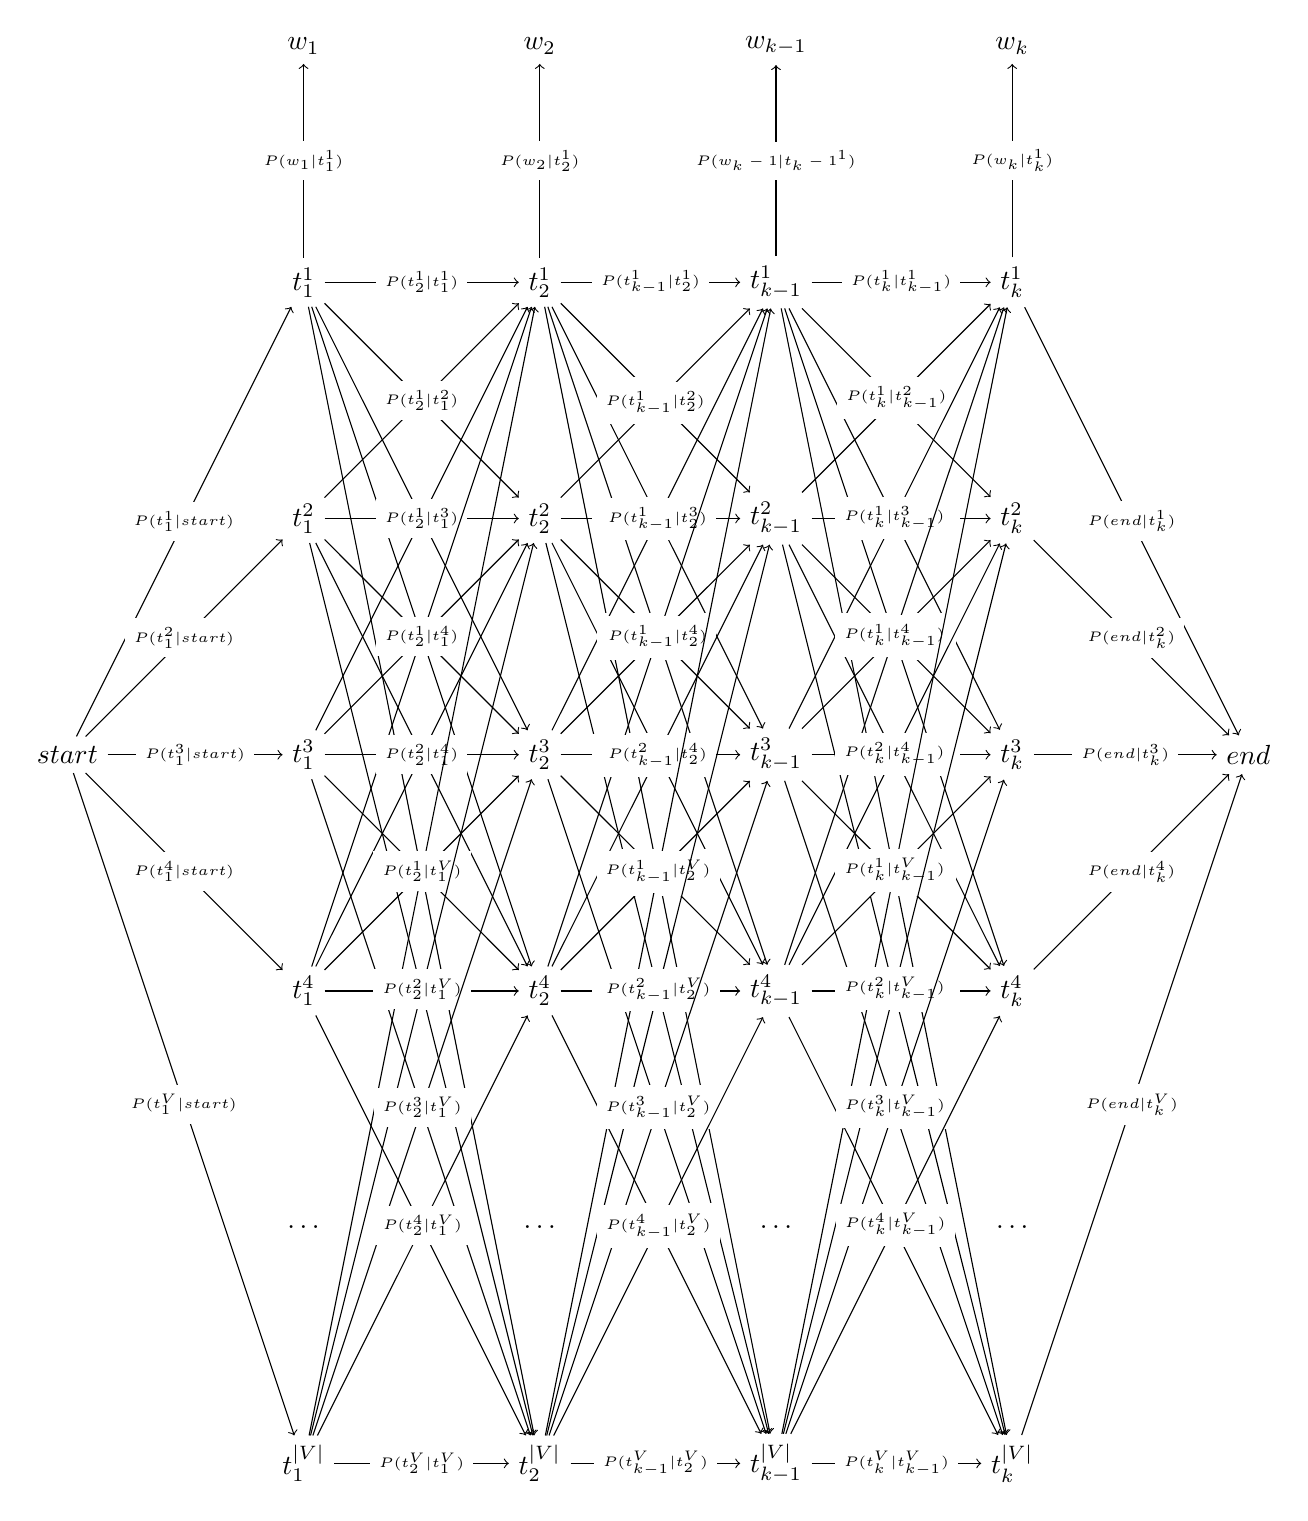
\begin{tikzpicture}[node distance=3cm]
\node(start)                           {$start$};

\node(t_1^3)	[right of=start]	{$t_1^3$};
\node(t_1^2)	[above of=t_1^3]	{$t_1^2$};
\node(t_1^1)	[above of=t_1^2]	{$t_1^1$};
\node(t_1^4)	[below of=t_1^3]	{$t_1^4$};
\node(t_1^dots)	[below of=t_1^4]	{$\ldots$};
\node(t_1^V)	[below of=t_1^dots]	{$t_1^{|V|}$};

\node(t_2^3)	[right of=t_1^3]	{$t_2^3$};
\node(t_2^2)	[above of=t_2^3]	{$t_2^2$};
\node(t_2^1)	[above of=t_2^2]	{$t_2^1$};
\node(t_2^4)	[below of=t_2^3]	{$t_2^4$};
\node(t_2^dots)	[below of=t_2^4]	{$\ldots$};
\node(t_2^V)	[below of=t_2^dots]	{$t_2^{|V|}$};

\node(t_k-1^3)	[right of=t_2^3]	{$t_{k-1}^3$};
\node(t_k-1^2)	[above of=t_k-1^3]	{$t_{k-1}^2$};
\node(t_k-1^1)	[above of=t_k-1^2]	{$t_{k-1}^1$};
\node(t_k-1^4)	[below of=t_k-1^3]	{$t_{k-1}^4$};
\node(t_k-1^dots)	[below of=t_k-1^4]	{$\ldots$};
\node(t_k-1^V)	[below of=t_k-1^dots]	{$t_{k-1}^{|V|}$};

\node(t_k^3)	[right of=t_k-1^3]	{$t_k^3$};
\node(t_k^2)	[above of=t_k^3]	{$t_k^2$};
\node(t_k^1)	[above of=t_k^2]	{$t_k^1$};
\node(t_k^4)	[below of=t_k^3]	{$t_k^4$};
\node(t_k^dots)	[below of=t_k^4]	{$\ldots$};
\node(t_k^V)	[below of=t_k^dots]	{$t_k^{|V|}$};

\node(w_1)	[above of=t_1^1]	{$w_1$};
\node(w_2)	[above of=t_2^1]	{$w_2$};
\node(w_k-1)	[above of=t_k-1^1]	{$w_{k-1}$};
\node(w_k)	[above of=t_k^1]	{$w_k$};

\node(end)	[right of=t_k^3]	{$end$};

\foreach \x in {1,2,3,4,V} {
	\draw [->] (start) -- (t_1^\x) node [midway, fill=white] {\tiny	$P(t_1^\x|start)$}; }

\foreach \x in {1,2,3,4,V} {
	\foreach \y in {1,2,3,4,V} {
		\draw [->] (t_1^\x) -- (t_2^\y) node [midway,fill=white]{\tiny $P(t_2^\y|t_1^\x)$};
	}
}

\foreach \x in {1,2,3,4,V} {
	\foreach \y in {1,2,3,4,V} {
		\draw [->] (t_2^\x) -- (t_k-1^\y) node [midway,
		fill=white]{\tiny $P(t_{k-1}^\y|t_2^\x)$};
	}
}

\foreach \x in {1,2,3,4,V} {
	\foreach \y in {1,2,3,4,V} {
		\draw [->] (t_k-1^\x) -- (t_k^\y) node [midway,
		fill=white]{\tiny $P(t_k^\y|t_{k-1}^\x)$};
	}
}

\foreach \x in {1,2,3,4,V} {
	\draw [->] (t_k^\x) -- (end) node [midway,
		fill=white]{\tiny $P(end|t_k^\x)$};
}

\foreach \x in {1,2,k-1,k} {
	\draw [->] (t_\x^1) -- (w_\x) node [midway,fill=white]{\tiny
	$P(w_\x|t_\x^1)$}; }

\end{tikzpicture}
\caption{Viterbi lattice}
\label{fig:latice}
\end{figure} 

To calculate the $V_j(t_j^i)$ of the Viterbi decoding we start from column $j=1$
and proceed to $j=k$.

To caclulate the ``probabilities'' $P(w_j|t_j^i)$ we use the a normalized
inverse Levenstein distance. More specificaly:

$$
P(w_j|t_j^i) = 1 - \frac{levenstein(w_j, t_j^i)}{max(length(w_j),
length(t_j^i)) + 1}
$$

We have used the maximum word length as the normalization parameter. This is due
to the fact that the maximum edit distance is the maximum word length. So two
words that have a large distance will have $P(w_j|t_j^i)\approx0$ while the same
words will have $P(w_j|t_j^i)\approx1$.

Starting from the first level of the HMM we calculate $V_1(t_1^i)$ for each word
$i$ of the vocabulary:

$$
V_1(t_1^i) = P(t_1^i|start)P(w_1|t_1^i)
$$

For the next levels we calculate:

$$
V_j(t_j^i) = P(w_j|t_j^i)\max_{t_{j-1}}P(t_j^i|t_{j-1})V_1(t_{j-1})
$$

Where $t_{j-1}$ is in the range $[t_{j-1}^1, t_{j-1}^{|V|}]$ and $V$ is the
vocabulary.

We have implemented the above functionality in a Python function in order to add
to the a bigram model the capability to correct errors on unseen text.

We extended the bigram model used in exercise of part 1. The model is trained on
the english corpus of the europarl data set which contains transcripts of the
european parliament. 

The data set contains a vocabulary of about 17,000 words. Given that the Viterbi
algorithm has complexity of $O(T*S^2)$ where $T$ is the length of the sentence
and $S$ is the number of states of the HMM we deem that the algorithm is too
slow for practical use as it requires more than 8,500,000,000 operations for an
average 30 word sentence. Also most of these operations include tasks like
calling a probability distribution function for data and calculation of the
Levenstein distance making each operation very time consuming.

We attempted to do some preprocessing of the data to speed up the calculations.
One option is to precalculate the Levenstein distance of all pairs of words in
the vocabulary which requires $O(|V|^2)$ space. Then we would use as states
$t_j$ only the vocabulary words that have low edit distance to $w_j$ The other
option is to precalculate the probabilities of state transitions
$P(t_j|t_{j-1})$ which again requires $O(|V|^2)$ space. Due to resource
limitations in the machine we executed the program, we opted to do no
preprocessing and calculate these values as required. To compensate for the poor
performance we experimented with short sentences of length 5-7 words.

In order to test our implementation we creted a test data set which contains
errors. We used the held out data (see part 1) of the europarl dataset as a
basis for this new dataset.

The Viterbi decoder can correct two types of erros. Errors of type 1 are
word modifications that create tokens that do not exist in the vacabulary. Type
2 errors are word modifications that create tokens that happen to exist in the
vocabulary.

We want to create both types of errors in the test data set. To create type 1
errors we randomly select a word in the dataset and randomly replace 1-3
characters with other random characters. We perform this for $10\%$ of the words
in the data set.

To create type 2 errors, we select a random word in the dataset. Then we replace
it with a randomly selected word from the vocabulary. We change this way $10\%$
of the dataset.

Then we feed each sentence along with the probability distribution of our bigram
model to the Vitterbi decoder and expect to get back a corrected sentence. For
each sentence now we have 3 versions, the basis from the held out data set, the
sentence with the errors from the test data set and the sentence corrected from
the Viterbi decoder.

We want evaluate the performance of the decoder. We will use a metric that
calculates the error correction rate $ECR$:

$$
ECR = 1 - \frac{mistakes in the corrected data}{mistakes in the data}
$$

An positive $ECR$ value means that the decoder has returned sentences that
contain less errors than in the test dataset while a negative value means that
the decoder has added more errors. It is possible for the decoder to insert new
errors since in order to correct type 2 errors it reevaluate the probability
even of words that exist in the vocabulary.

Due to the performance limitations stated above we haven't executed this metric
for all the test data set but only for short sentence samples so we cannot make
a statement about it's actual performance. A few examples:

\begin{center}
  \begin{tabular}{ l | c | c }
    \hline
    data & sentence 1 & sentence 2\\ \hline
    original sentence & the debate is closed. & the vote will take place on
    thursday \\
    \hline test sentence & the debate io closed. & she excessively wil take
    place on thursday\\
    \hline corrected sentence & the debate is closed. & she excessively will
    take place on thursday\\
    \hline\hline
    data & sentence 3 &\\ \hline
    original sentence & but where will you place the emphasis? & \\ \hline
    test sentence & but wheree will need place he emphasis? & \\ \hline
    corrected sentence & but where will need place the emphasis? & \\ \hline
  \end{tabular}
\end{center}


\end{document}
